\documentclass[tikz,border=10pt]{standalone}
\usepackage{fontspec}
\usepackage{tikz}
\usetikzlibrary{arrows.meta,calc,positioning}

\setmainfont[
  Path=C:/Windows/Fonts/,
  UprightFont=GOTHIC.TTF,
  BoldFont=GOTHICB.TTF,
  ItalicFont=GOTHICI.TTF,
  BoldItalicFont=GOTHICBI.TTF
]{Century Gothic}

\definecolor{navy}{HTML}{0C171F}
\definecolor{green}{HTML}{00F700}

\tikzset{
  card/.style={
    draw=navy,
    line width=0.95pt,
    rounded corners=5pt,
    minimum width=5.2cm,
    minimum height=2.05cm,
    text width=4.65cm,
    align=center,
    text=navy,
    fill=none,
    font=\fontsize{12}{14.5}\selectfont
  },
  result/.style={
    card,
    minimum width=6.0cm,
    text width=5.45cm
  },
  rowlabel/.style={
    text=navy,
    font=\bfseries\fontsize{10.5}{12.5}\selectfont,
    align=left,
    text width=3.0cm,
    anchor=west
  },
  primary/.style={
    text=navy,
    font=\bfseries\fontsize{13}{16}\selectfont,
    align=center
  },
  secondary/.style={
    text=navy,
    font=\fontsize{10.5}{13}\selectfont,
    align=center
  },
  flow/.style={
    -{Latex[length=3.0mm,width=2.0mm,fill=green]},
    draw=navy,
    line width=1.0pt
  },
  same/.style={
    draw=green,
    line width=1.0pt,
    dashed
  },
  samelabel/.style={
    text=green,
    font=\bfseries\fontsize{10.5}{12.5}\selectfont,
    align=center
  }
}

\begin{document}
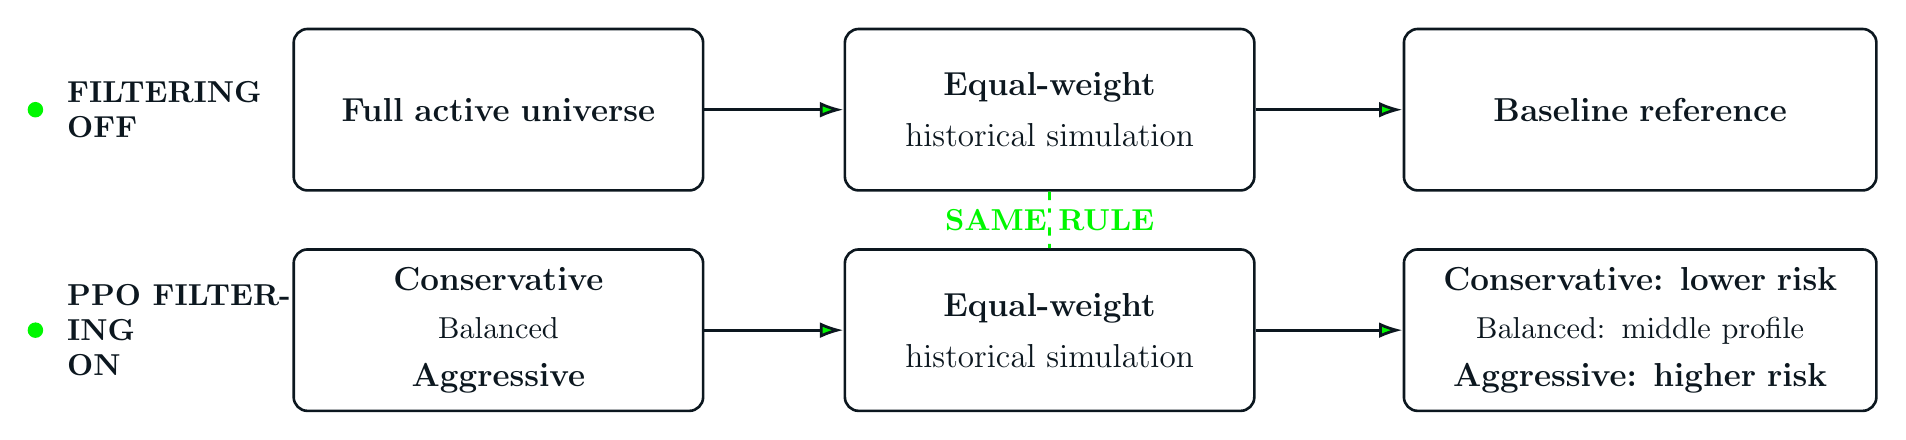
\begin{tikzpicture}[x=1cm,y=1cm]
  % Row labels
  \fill[green] (0.12,4.25) circle (2.8pt);
  \node[rowlabel] at (0.40,4.25) {FILTERING OFF};

  \fill[green] (0.12,1.45) circle (2.8pt);
  \node[rowlabel] at (0.40,1.45) {PPO FILTERING\\ON};

  % Baseline path
  \node[card] (full) at (6.0,4.25)
    {\textbf{\fontsize{13}{16}\selectfont Full active universe}};

  \node[card] (ruleTop) at (13.0,4.25)
    {\textbf{\fontsize{13}{16}\selectfont Equal-weight}\\[4pt]
     historical simulation};

  \node[result] (baseline) at (20.5,4.25)
    {\textbf{\fontsize{13}{16}\selectfont Baseline reference}};

  % PPO-filtered path
  \node[card] (profiles) at (6.0,1.45)
    {\textbf{\fontsize{13}{16}\selectfont Conservative}\\[3pt]
     {\fontsize{10.5}{13}\selectfont Balanced}\\[3pt]
     \textbf{\fontsize{13}{16}\selectfont Aggressive}};

  \node[card] (ruleBottom) at (13.0,1.45)
    {\textbf{\fontsize{13}{16}\selectfont Equal-weight}\\[4pt]
     historical simulation};

  \node[result] (outcomes) at (20.5,1.45)
    {\textbf{\fontsize{12}{14.5}\selectfont Conservative: lower risk}\\[3pt]
     {\fontsize{10.5}{13}\selectfont Balanced: middle profile}\\[3pt]
     \textbf{\fontsize{12}{14.5}\selectfont Aggressive: higher risk}};

  % Same evaluation flow in both paths
  \draw[flow] (full.east) -- (ruleTop.west);
  \draw[flow] (ruleTop.east) -- (baseline.west);
  \draw[flow] (profiles.east) -- (ruleBottom.west);
  \draw[flow] (ruleBottom.east) -- (outcomes.west);

  \draw[same] (ruleTop.south) -- ($(ruleTop.south)!0.37!(ruleBottom.north)$);
  \draw[same] ($(ruleTop.south)!0.63!(ruleBottom.north)$) -- (ruleBottom.north);
  \node[samelabel]
    at ($(ruleTop.south)!0.5!(ruleBottom.north)$) {SAME RULE};
\end{tikzpicture}
\end{document}
